\documentclass[twoside]{article}

\usepackage{aistats2027}
\usepackage{amsmath,amssymb,amsfonts,amsthm}
\usepackage{booktabs}
\usepackage{enumitem}
\usepackage{graphicx}
\usepackage{microtype}
\usepackage{xcolor}
\usepackage{hyperref}
\usepackage{url}

\newcommand{\method}{PCPI}
\newcommand{\E}{\mathbb E}
\newcommand{\R}{\mathcal R}
\newcommand{\Acal}{\mathcal A}
\newcommand{\Dcal}{\mathcal D}
\newcommand{\ours}{\textsc{Full}}
\newcommand{\nollm}{\textsc{No-LLM}}
\newcommand{\single}{\textsc{Single}}
\newtheorem{proposition}{Proposition}

\begin{document}

\twocolumn[
\aistatstitle{Protected Bayesian Discovery with Lineage-Bound LLM Synthesis}
\aistatsauthor{Anonymous Authors}
\aistatsaddress{Anonymous Institution}
]

\begin{abstract}
Large language models can propose scientific hypotheses, but a fluent proposal
is not evidence that a model should enter a scientific posterior or control the
next experiment. We introduce \method{}, a protected Bayesian framework for
combining heterogeneous symbolic-discovery engines with a language model.
The language model cannot freely author an accepted law: it emits typed
composition directives that reference immutable engine lineages, and a
deterministic compiler constructs the resulting support. Candidate sources
are admitted by out-of-fold predictive evidence, with at least half of the
prior mass reserved for a registered core and automatic fallback whenever any
arbitration fold indicates negative transfer. The admitted bank is partitioned
into operational predictive-equivalence classes and measurements are ranked by
certified reduction in Bayes decision risk, not expression novelty or
predictive variance alone.

Two fresh, matched-engine synthesis screens over four symbolic-regression
families complete all 32 condition runs without failure. Holding engine
execution fixed, lineage-bound synthesis improves normalized expected-risk
AULC by \(0.0192\) and \(0.0328\), with nonnegative family effects in both
screens and positive effects in two and three families, respectively. On a
measured gas-turbine source screen, protected stacking assigns weights
\(0.511/0.489/{\approx}0\) to core/LLM/MCTS sources and rejects the redundant
engine. A fixed-prefix replay produces 23 positive and 23 distinct risk-AULC
values among 32 completed rows, resolving an earlier zero-signal metric.
Crucially, a matched-budget realized pilot is negative
(predicted--realized correlation \(-0.575\)); the calibrated deployment policy
therefore authorizes acquisition only for the material-science family and
authorizes no family for unconditional LLM synthesis. These results support
selective hypothesis synthesis and fail-closed deployment, not universal LLM
superiority.
\end{abstract}

\section{Introduction}

Modern scientific-discovery systems can call symbolic regression engines,
program synthesizers, and large language models (LLMs) to generate candidate
laws. This expands the search space, but also creates a statistical problem:
adding a seemingly intelligent source can degrade the hypothesis bank,
collapse useful uncertainty, or select an experiment whose modeled value does
not materialize. Standard leaderboards largely evaluate the final equation;
they do not specify when a new proposal source should be trusted, how
conflicting sources should be combined, or when the system should abstain.

We study a narrower and testable notion of an AI scientist. Multiple engines
produce auditable candidate lineages. An LLM may synthesize structures across
these lineages, but it cannot directly assign posterior mass or authorize an
experiment. A protected Bayesian layer decides which sources enter the bank,
and a decision-theoretic layer decides whether the bank supports a
measurement. We call the resulting framework \method{}.

The central distinction is between \emph{proposal intelligence} and
\emph{statistical authority}. The LLM is useful when it composes complementary
structural evidence that individual engines miss. Statistical authority
remains with a normalized finite posterior, out-of-fold source admission, and
a registered Bayes-risk objective. This separation also makes negative
evidence actionable: a source can remain in the provenance ledger while
receiving zero production mass.

Our contributions are:
\begin{enumerate}[leftmargin=*,itemsep=2pt,topsep=3pt]
  \item \textbf{Lineage-bound LLM synthesis.} The LLM emits typed set
  operations over verified parent lineages. A deterministic compiler rejects
  unknown parents, unsupported grammar, duplicate support, and synthesis
  without structural novelty.
  \item \textbf{Protected Bayesian source admission.} Sources are evaluated
  on independent arbitration folds. Harmful sources are removed before
  stacking, at least half of production prior mass remains on a registered
  core, and a dyadic shrinkage path returns to the core until every fold is
  noninferior.
  \item \textbf{Operational decision-risk design.} The scientific estimand is
  a frozen predictive-equivalence class. Candidate measurements are selected
  by a certified lower bound on expected reduction in Bayes class-decision
  risk. Unresolved ranking or a nonviable bank stops measurement.
  \item \textbf{Claim-calibrated evaluation.} Matched-engine screens isolate
  the synthesis contribution. Response-free replay tests risk resolution;
  realized trajectories separately test deployment. The resulting policy is
  deliberately selective: strong expected-risk evidence does not override
  negative realized evidence.
\end{enumerate}

This is not a claim that an LLM should generally schedule more engines. Our
allocation experiments do not establish that claim. Instead, the current
evidence supports a more specific mechanism: an LLM can synthesize useful
cross-engine hypotheses, while a protected statistical layer decides whether
those hypotheses are safe to use.

\section{Related Work}

\paragraph{Symbolic scientific discovery.}
Genetic programming, physics-guided decomposition, neural symbolic regression,
and modern systems such as PySR search over expressions using predictive fit
and complexity \cite{koza1992gp,udrescu2020aifeynman,
petersen2021deepsymbolic,cranmer2023pysr}. Our focus is not a new base search
engine. We combine heterogeneous engines while preserving source identity and
make the downstream scientific decision depend on operational behavior rather
than expression syntax.

\paragraph{LLMs for equation and program discovery.}
LLM-SR uses language models to generate executable equation-discovery
programs \cite{shojaee2024llmsr}; FunSearch couples language-model proposals
with an automatic evaluator \cite{romeraparedes2024funsearch}; broader AI
scientist systems use language models for planning and iterative research
\cite{lu2024aiscientist,gotts2025coscientist}. These works demonstrate that
language models can be productive proposal mechanisms. \method{} addresses a
different question: how can an LLM combine evidence from multiple registered
engines without becoming the authority that accepts its own hypothesis?
Our typed compiler only permits operations over supplied lineage identifiers,
and survival is decided by independent predictive evidence.

\paragraph{Stacking and safe improvement.}
Predictive stacking combines models by optimizing out-of-sample log score
\cite{yao2018stacking}; hierarchical variants allow context-dependent
combinations \cite{yao2022hierarchical}. Conservative policy-improvement
methods retain a baseline unless an alternative is sufficiently supported
\cite{laroche2019spibb,katariya2019interleaving}. We combine these ideas at
the \emph{proposal-source} level: individually harmful sources are removed,
the core retains a fixed reserve, and all admitted candidates remain discrete
scientific hypotheses rather than being averaged into one predictor.

\paragraph{Bayesian experimental design.}
Bayesian experimental design selects actions by expected utility
\cite{chaloner1995bayesian}. Prediction-oriented active learning emphasizes
that model information and predictive value need not coincide
\cite{bickfordsmith2023prediction}. We use expected reduction in Bayes
decision risk for a frozen operational-class estimand and require a numerical
ranking certificate before a candidate response can be opened.

\paragraph{Quality diversity.}
MAP-Elites and quality-diversity (QD) algorithms retain high-quality solutions
across behavioral niches \cite{mouret2015mapelites}. QD has also been applied
to symbolic regression \cite{trujillo2025qdsr}. Our optional Bayesian
operational-QD archive uses a descriptor derived from a candidate's
decision-risk profile, rejects predictively unsafe candidates, and hands over
to a QD repertoire only when fixed-prefix noninferiority is certified.

\section{Problem Formulation}

\subsection{Hypotheses, sources, and immutable lineages}

Let \(H_0=\{(x_i,y_i)\}_{i=1}^{n_0}\) be the initial development history.
A proposal source \(s\in\mathcal S\) emits symbolic hypotheses
\(h=(e,\ell,s)\), where \(e\) is an expression and \(\ell\) is an immutable
lineage identifier. The registered core source \(s_0\) contains deterministic
anchors and cannot be removed. Optional sources include symbolic engines and
the LLM synthesis source.

Each expression is compiled into a closed linear-in-coefficients support
\(\phi_h(x)\). With a Gaussian--inverse-Gamma prior,
\[
 y=\phi_h(x)^\top\theta_h+\epsilon,\qquad
 \epsilon\sim\mathcal N(0,\sigma_h^2),
\]
the coefficient and noise parameters are integrated analytically. This gives
an exact finite posterior over the frozen bank,
\[
 p(h\mid H_0)\propto p(h)\,p(y_{1:n_0}\mid X_{1:n_0},h).
\]
Fitted coefficients produced during search are discarded and refit under this
common posterior contract.

\subsection{Operational scientific estimand}

Expression identity is often too fine: different symbolic forms can be
indistinguishable on the action domain relevant to a scientific decision.
Before sequential measurement, we freeze an action set
\(\Acal_0=\{a_1,\ldots,a_M\}\), a predictive distance, and a resolution.
These define a map
\[
 C=g_{H_0}(h)\in\{1,\ldots,K\}
\]
from symbolic laws to operational predictive-equivalence classes. The class
posterior is the pushforward
\[
 p_t(c)=\sum_{h:g_{H_0}(h)=c}p_t(h).
\]
All policies compared at a coordinate use the same frozen map and initial
posterior.

For \(0\)--\(1\) class loss, the Bayes risk is
\[
 \R(p_t)=1-\max_c p_t(c).
\]
The ideal utility of action \(a\) is expected decision-risk reduction,
\begin{equation}
 U_t(a)=\R(p_t)-
 \E_{Y_a\sim p_t(\cdot\mid a)}
 \left[\R\!\left(p_{t+1}(\cdot\mid a,Y_a)\right)\right].
 \label{eq:riskutility}
\end{equation}
This targets the terminal scientific decision directly. It is not predictive
variance and need not agree with expression-recovery accuracy.

\section{Method}

\subsection{Typed lineage-bound synthesis}

After the engines run, the LLM receives a structured evidence registry. It may
return a directive
\[
 d=(o,\ell_1,\ldots,\ell_m,r),
\]
where \(o\) is one of \textsc{UnionSupports},
\textsc{IntersectionSupports}, or \textsc{AugmentBase}; the \(\ell_j\) are
existing lineage identifiers; and \(r\) is an auditable rationale. The
provider does not return the accepted expression.

A deterministic compiler parses the parent expressions into structural
support sets \(T(\ell_j)\), applies the typed set operation, adds an intercept
if needed, and constructs a canonical expression from registered parent
terms. It rejects the directive if a parent is unknown, a term is outside the
closed grammar, fewer than two parent lineages are referenced, the output has
fewer than two supports, or the output support equals a parent support.
The synthesized identity is a hash of the operation, ordered parents, and
compiled support.

\begin{proposition}[Provenance closure]
Every accepted synthesized support is a deterministic function of registered
parent lineages and the finite operation vocabulary. Changing free-form
rationale while holding the typed directive fixed cannot change the compiled
hypothesis.
\end{proposition}

The proposition follows directly from canonical parsing and hash-bound
compilation. It is modest but important: the LLM contributes a structural
composition decision, not unverifiable coefficients or hidden evidence.

\subsection{Independent source admission}

Let \(z_{is}\) be the log posterior-predictive density assigned by source
\(s\) to arbitration observation \(i\), computed after fitting only on
\(H_0\). Arbitration observations are split into folds
\(\Dcal_1,\Dcal_2\). Relative to the core \(s_0\), define
\[
 G_{ks}=\sum_{i\in\Dcal_k}(z_{is}-z_{is_0}).
\]
A source is eligible only if every fold is nonnegative up to a
floating-point containment tolerance. This individual check prevents a
strong source from masking a harmful one inside a mixture.

For the remaining sources, unconstrained stacking chooses
\[
 \widetilde w=\arg\max_{w\in\Delta}
 \sum_i \log\!\left(\sum_s w_s\exp z_{is}\right).
\]
We then reserve at least half of production prior mass for the core. Along
the fixed dyadic path
\[
 w(\alpha)=\alpha\widetilde w+(1-\alpha)e_{s_0},
 \qquad
 \alpha\in\{2^{-1},\ldots,2^{-8},0\},
\]
we select the largest \(\alpha\) for which every fold's mixture log-score is
noninferior to the core. Rejected sources remain in the provenance ledger
with zero mass and a fold-level certificate.

\begin{proposition}[Fold-wise core protection]
For the selected \(w(\alpha)\), the registered arbitration log score is no
worse than the core on every fold, up to the declared numerical containment
tolerance. If no optional mixture satisfies the condition, the procedure
returns \(e_{s_0}\).
\end{proposition}

This is an arbitration guarantee, not a population no-harm theorem. Its role
is to make the deployment boundary explicit and testable.

\subsection{Certified decision-risk selection}

For each candidate action, adaptive integration returns an interval
\([L_t(a),R_t(a)]\) containing the computed utility in
Eq.~\eqref{eq:riskutility}. An action is released only when one lower bound
exceeds every competing upper bound by a registered numerical tolerance.
Otherwise the system abstains or executes the registered reference policy.
The decision is persisted before one matching response is opened.

For short-prefix screening, we evaluate risks after \(0,8,16,\) and \(32\)
responses and report normalized risk-reduction AULC. The prefixes and
normalization are frozen before evaluating a condition. This repaired an
earlier binary-readiness statistic that was identically zero across many
rows.

\subsection{Optional operational quality diversity}

The operational-QD archive uses
\[
\begin{aligned}
b(h)=\big(&b_{\rm lead}(h),\,b_{\rm concentration}(h),\\[-2pt]
          &b_{\rm support}(h)\big)
\end{aligned}
\]
as a behavior descriptor. Within a cell, verified candidates are ordered by
certified risk lower bound, predictive quality, lower complexity, and stable
identity. Unsafe candidates cannot enter the archive. A QD repertoire
replaces the legacy bank only if its lower-bound curve is noninferior at all
fixed prefixes and its AULC is strictly larger; otherwise the legacy bank is
retained.

\section{Experimental Protocol}

\paragraph{Conditions.}
\ours{} contains the same registered symbolic engines as \nollm{} plus typed
LLM synthesis. \nollm{} contains all deterministic and engine proposals but
no LLM candidates. \single{} is the registered single-engine control. In
the synthesis-only comparisons, engine executions, budgets, seeds, and raw
engine candidates are identity-matched within every pair.

\paragraph{Data.}
The primary synthesis screens use fresh development tasks from four
LLM-SRBench families: biological population growth, chemical reactions,
transformed physical laws, and materials science. Each screen uses one task
per family and two seeds, yielding 16 condition rows or eight paired
comparisons. The measured source-admission case uses UCI gas-turbine CO.
No synthesis screen opens candidate-action, test, OOD, or held-out responses.

\paragraph{Metrics and claims.}
The synthesis metric is normalized fixed-prefix expected-risk AULC; it is
model-relative development evidence. The realized pilot separately opens
two selected development responses after each durable decision and compares
targeted acquisition with a matched random policy. Family authorization uses
a Jeffreys prior on binary task-level success and a preregistered 90\% lower
credible bound. Every failure and unresolved task remains in the analysis.
No result in this paper is untouched-heldout confirmation.

\begin{figure*}[t]
\centering
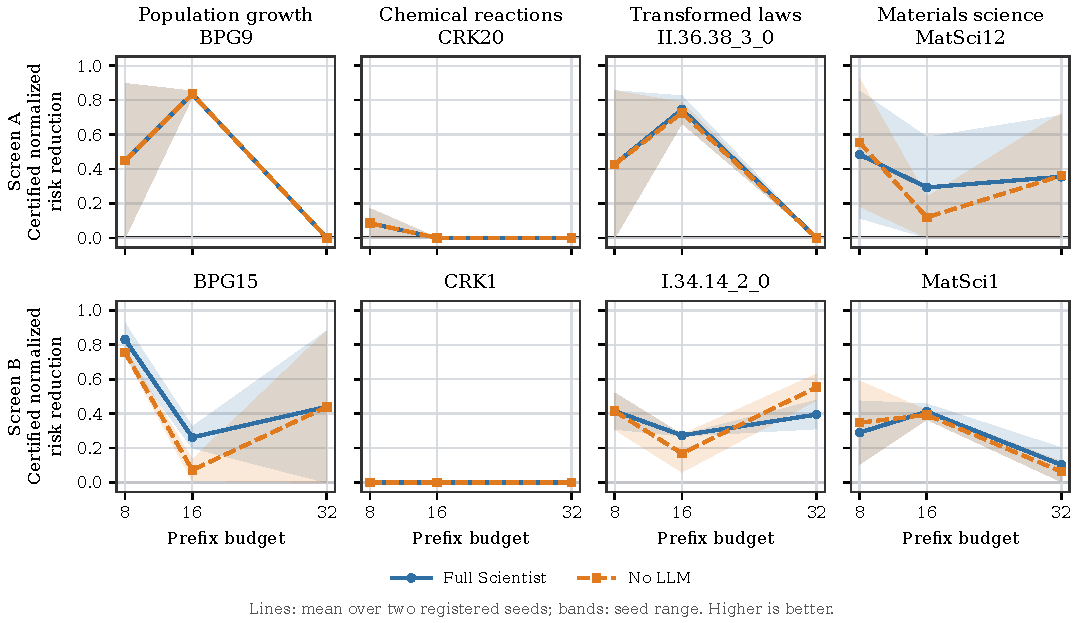
\includegraphics[width=\textwidth]{figures/pcpi_prefix_curves.pdf}
\caption{\textbf{Response-free fixed-prefix decision-risk curves.}
Rows are two prospectively frozen fresh-task screens and columns are scientific
families. Lines show means over two registered seeds; shaded regions show the
seed range, not confidence intervals. \ours{} and \nollm{} have identical
engine executions within every pair. Higher is better. Candidate-action,
test, OOD, and held-out responses remain closed.}
\label{fig:prefix-curves}
\end{figure*}

\section{Results}

\subsection{LLM synthesis adds expected-risk value under matched engines}

Figure~\ref{fig:prefix-curves} reports two fresh synthesis-only screens. Both
complete all 16 rows with zero failures, identical engine execution within
every pair, structurally novel LLM candidates in all four families, and no
negative family-level effect. Mean \ours{}--\nollm{} AULC is \(0.0192\) in
Screen~A and \(0.0328\) in Screen~B. The first screen is positive in
transformed-law and materials tasks; the second is positive in population,
transformed-law, and materials tasks and tied in chemistry.

Because engines and engine outputs are matched, the contrast isolates the
typed synthesis layer rather than additional search compute. It does not,
however, prove realized benefit after observing new responses.

\subsection{Protected admission keeps useful sources and rejects others}

On the gas-turbine CO source screen, the unconstrained stacking solution places
approximately \(97.8\%\) mass on LLM candidates and negligible mass on MCTS.
After the fixed core reserve, the production weights are
\(0.511\) core, \(0.489\) LLM, and \(6.6\times10^{-17}\) MCTS. The resulting
mixture improves fold log score by \(5.23\) and \(3.01\) nats over the core.
The hypothesis bank retains five operational classes with entropy \(0.538\)
nats. This example demonstrates the intended asymmetry: engines and the LLM
may propose broadly, but an optional source receives production mass only
when it contributes independent predictive evidence.

\subsection{Risk scoring is functional, but realized transfer is selective}

The response-free fixed-prefix replay accounts for 32 of 36 registered rows
(four source artifacts are absent), with no outer replay exception or
log-mass failure. It yields 23 positive AULCs and 23 distinct AULC values,
showing that the repaired risk score is not the earlier constant-zero signal.

The stronger realized test is less favorable. All 32 matched trajectories
complete without failure, but the mean symmetric synthesis effect is
\(-0.0827\), the mean acquisition effect is \(-0.00019\), and the
predicted--realized correlation is \(-0.575\). A familywise calibration over
eight development tasks therefore authorizes decision-risk acquisition only
for materials science: its posterior success mean is \(0.833\) with 90\%
lower bound \(0.552\). No family is authorized for unconditional synthesis
deployment.

\begin{figure*}[t]
\centering
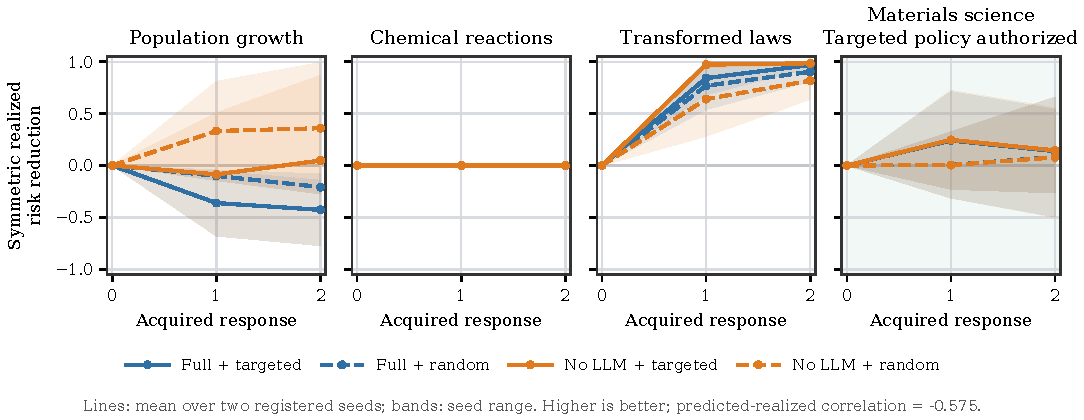
\includegraphics[width=\textwidth]{figures/pcpi_realized_trajectories.pdf}
\caption{\textbf{Matched-budget realized decision-risk trajectories.}
Each panel is a scientific family; lines are means over two registered seeds
and bands are seed ranges. Solid curves use targeted acquisition and dashed
curves use matched random acquisition. Higher is better. The pale materials
panel is the only family authorized by the preregistered realized-policy
calibration. All 32 trajectories completed, but the pooled
predicted--realized correlation is \(-0.575\), so no global superiority claim
is made.}
\label{fig:realized-curves}
\end{figure*}

\begin{table*}[t]
\caption{Evidence layers and the claims they authorize.}
\label{tab:claims}
\centering
\small
\begin{tabular}{p{0.17\textwidth}p{0.13\textwidth}p{0.61\textwidth}}
\toprule
Layer & Outcome & Authorized claim\\
\midrule
Matched synthesis & Pass & LLM synthesis improves model-relative expected-risk AULC on screened tasks.\\
Source admission & Pass & Optional sources can be retained or zeroed without candidate-response access.\\
Prefix replay & Pass & Repaired risk signal is finite, varying, and nonconstant.\\
Realized pilot & Fail & No global realized superiority claim.\\
Family calibration & Selective & MatSci acquisition only; no synthesis family.\\
BOQD replay & Mixed & Safe fallback; cross-family benefit unproved.\\
\bottomrule
\end{tabular}
\end{table*}

This separation is a feature of the method rather than an inconvenient
postscript. A system that used response-free gains as automatic deployment
authority would have made an unsupported broad claim; \method{} instead turns
the realized negative result into an explicit abstention policy.

\subsection{Operational QD is correct and safe, but not yet broadly effective}

The operational-QD algebraic gate verifies that different risk profiles occupy
different cells, a same-cell challenger must improve certified quality, unsafe
candidates are rejected, and emitter credit is based on independent tasks.
In raw replay, BOQD has positive mean effect \(0.0175\) but negative effects
for transformed-law and materials families. Conservative handover removes
all observed negative family effects and increases the mean to \(0.0463\), but
only population growth remains positive (\(0.1852\)); the other three families
fall back to the legacy bank. BOQD is therefore an algorithmically valid
auxiliary mechanism, not yet a cross-family efficacy result.

\section{Discussion}

\paragraph{What is new?}
LLM equation generation, predictive stacking, Bayesian experimental design,
and QD each have substantial prior work. The contribution is their
statistically separated composition: (i) the LLM can only propose a typed
operation over immutable multi-engine evidence; (ii) individually harmful
sources are removed before a core-reserved stack is formed; and (iii)
experiment selection targets a frozen scientific decision and can fail
closed. The matched-engine ablation is essential because it attributes gains
to synthesis rather than additional engine calls.

\paragraph{Why expected and realized effects differ.}
Decision-risk utilities are conditional on the hypothesis bank and predictive
model. A score can be numerically correct for that model and still transfer
poorly when the bank omits the relevant mechanism or its predictive
uncertainty is misspecified. The negative correlation in the realized pilot
is direct evidence of this boundary. It motivates calibrated familywise
deployment rather than another result-fitted score.

\paragraph{Limitations.}
The positive synthesis evidence is development-only and compares against
internal ablations, not all external symbolic-regression systems. The number
of tasks per family is small. No untouched confirmation set has been opened.
The current production posterior is a finite conjugate bank; the repository's
open-grammar SMC work is correctness-only and is not claimed as part of these
experiments. BOQD lacks cross-family efficacy. Finally, \method{} provides
an empirical fold-safety certificate, not a distribution-free no-harm
guarantee.

\section{Conclusion}

\method{} separates scientific creativity from statistical authority.
Heterogeneous engines produce immutable evidence lineages; an LLM composes
them through a typed deterministic interface; protected Bayesian admission
decides which sources receive mass; and certified decision-risk reduction
decides whether to measure. Matched-engine experiments support the specific
claim that LLM synthesis can improve response-free expected-risk AULC.
Realized experiments do not support universal superiority, and the framework
correctly restricts deployment. We view this selective result as the right
standard for an auditable AI scientist: propose broadly, verify independently,
and abstain when modeled value does not transfer.

\section*{AI Use Statement}

Large language models were used as research software components in the
evaluated method and were also used for code assistance, literature discovery,
and language editing during manuscript preparation. All mathematical claims,
citations, source code, experiment registrations, and result artifacts were
checked by the authors. Manuscript-writing tools did not receive protected
candidate, test, OOD, or held-out responses. In the evaluated system, provider
outputs were restricted by typed contracts and could not directly assign
posterior mass, open a response, or authorize a scientific claim.

\bibliographystyle{plain}
\bibliography{references}

\clearpage
\appendix

\section{Exact Finite-Bank Posterior}

For a frozen support \(h\), let \(\Phi_h\) be its design matrix and use
\[
\theta_h\mid\sigma^2\sim
\mathcal N(m_0,\sigma^2\Lambda_0^{-1}),\qquad
\sigma^2\sim\operatorname{IG}(\alpha_0,\beta_0).
\]
Then
\[
\begin{aligned}
\Lambda_n&=\Lambda_0+\Phi_h^\top\Phi_h,\\
m_n&=\Lambda_n^{-1}(\Lambda_0m_0+\Phi_h^\top y),\\
\alpha_n&=\alpha_0+n/2,\\
\beta_n&=\beta_0+\tfrac12(y^\top y+m_0^\top\Lambda_0m_0-
m_n^\top\Lambda_nm_n).
\end{aligned}
\]
The collapsed marginal is
\begin{align*}
\log p(y\mid h)
={}&-\frac n2\log(2\pi)
+\frac12(\log|\Lambda_0|-\log|\Lambda_n|)\\
&+\alpha_0\log\beta_0-\alpha_n\log\beta_n\\
&+\log\Gamma(\alpha_n)-\log\Gamma(\alpha_0).
\end{align*}
All search-produced coefficients are discarded before this common refit.

\section{Source Admission Details}

Individual source admission precedes mixture optimization. For every optional
source, the implementation records fold gains, numerical tolerances,
admission status, zero production mass when rejected, and whether a negative
fold certifies negative transfer. A structurally duplicate source can instead
receive a redundancy certificate. Conditional engine admission evaluates an
engine against the already retained core--LLM reference, preventing a
redundant engine from receiving credit for an improvement already supplied by
the LLM.

\section{Additional Experimental Accounting}

\begin{table}[h]
\caption{Claim boundaries of the principal artifacts.}
\centering
\small
\begin{tabular}{p{0.30\linewidth}p{0.60\linewidth}}
\toprule
Artifact & Boundary\\
\midrule
Synthesis-only v2/v3 & Fresh-task, response-free development screens; no realized or confirmation claim.\\
Gas source admission & Initial-data and arbitration responses only; no acquisition response.\\
Fixed-prefix replay & Historical-candidate functionality; engines and LLM not rerun.\\
Realized DRR pilot & Development responses opened after durable selection; held-out closed.\\
Policy calibration & Familywise deployment decision; not universal superiority.\\
BOQD correctness & Algebra and archive behavior only; no real-data efficacy.\\
\bottomrule
\end{tabular}
\end{table}

The earlier 270-row formal DRR run is not used as positive evidence. It
contains 118 failures and a zero primary effect, motivating the fixed-prefix
repair. Similarly, historical PCPI acquisition stages that passed execution
but failed efficacy are preserved as negative evidence and are not pooled into
the positive synthesis results.

\end{document}
